\documentclass[14pt]{extbook}
\usepackage{multicol, enumerate, enumitem, hyperref, color, soul, setspace, parskip, fancyhdr} %General Packages
\usepackage{amssymb, amsthm, amsmath, latexsym, units, mathtools} %Math Packages
\everymath{\displaystyle} %All math in Display Style
% Packages with additional options
\usepackage[headsep=0.5cm,headheight=12pt, left=1 in,right= 1 in,top= 1 in,bottom= 1 in]{geometry}
\usepackage[usenames,dvipsnames]{xcolor}
\usepackage{dashrule}  % Package to use the command below to create lines between items
\newcommand{\litem}[1]{\item#1\hspace*{-1cm}\rule{\textwidth}{0.4pt}}
\pagestyle{fancy}
\lhead{Progress Quiz 3}
\chead{}
\rhead{Version ALL}
\lfoot{3012-8528}
\cfoot{}
\rfoot{Summer C 2021}
\begin{document}

\begin{enumerate}
\litem{
Find the equation of the line described below. Write the linear equation in the form $ y=mx+b $ and choose the intervals that contain $m$ and $b$.\[ \text{Perpendicular to } 3 x + 4 y = 15 \text{ and passing through the point } (8, 10). \]\begin{enumerate}[label=\Alph*.]
\item \( m \in [-1.82, -1.19] \hspace*{3mm} b \in [19.7, 22.4] \)
\item \( m \in [0.87, 1.78] \hspace*{3mm} b \in [-1.9, -0.6] \)
\item \( m \in [0.87, 1.78] \hspace*{3mm} b \in [-0.3, 1.1] \)
\item \( m \in [0.87, 1.78] \hspace*{3mm} b \in [1.9, 3] \)
\item \( m \in [-0.26, 0.92] \hspace*{3mm} b \in [-1.9, -0.6] \)

\end{enumerate} }
\litem{
Solve the equation below. Then, choose the interval that contains the solution.\[ -11(12x + 4) = -3(13x -5) \]\begin{enumerate}[label=\Alph*.]
\item \( x \in [-0.96, -0.63] \)
\item \( x \in [-0.1, 0.58] \)
\item \( x \in [-0.28, -0.02] \)
\item \( x \in [-0.61, -0.2] \)
\item \( \text{There are no real solutions.} \)

\end{enumerate} }
\litem{
Write the equation of the line in the graph below in Standard Form $Ax+By=C$. Then, choose the intervals that contain $A, B, \text{ and } C$.
\begin{center}
    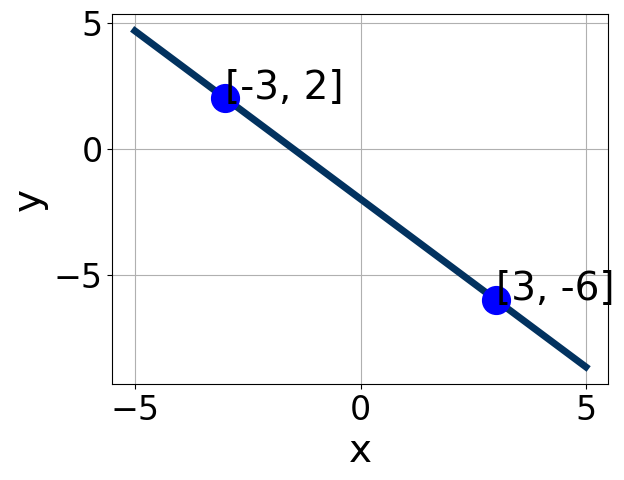
\includegraphics[width=0.5\textwidth]{../Figures/linearGraphToStandardCopyA.png}
\end{center}
\begin{enumerate}[label=\Alph*.]
\item \( A \in [2, 6], \hspace{3mm} B \in [2.44, 4.14], \text{ and } \hspace{3mm} C \in [-6.2, -4.4] \)
\item \( A \in [-8, -2], \hspace{3mm} B \in [-4.02, -2.76], \text{ and } \hspace{3mm} C \in [2.9, 8] \)
\item \( A \in [-2.67, 3.33], \hspace{3mm} B \in [0.8, 2.59], \text{ and } \hspace{3mm} C \in [-4.7, -0.7] \)
\item \( A \in [2, 6], \hspace{3mm} B \in [-4.02, -2.76], \text{ and } \hspace{3mm} C \in [2.9, 8] \)
\item \( A \in [-2.67, 3.33], \hspace{3mm} B \in [-1.55, -0.2], \text{ and } \hspace{3mm} C \in [0.4, 5] \)

\end{enumerate} }
\litem{
Find the equation of the line described below. Write the linear equation in the form $ y=mx+b $ and choose the intervals that contain $m$ and $b$.\[ \text{Parallel to } 9 x + 4 y = 10 \text{ and passing through the point } (6, -8). \]\begin{enumerate}[label=\Alph*.]
\item \( m \in [-4.25, -1.25] \hspace*{3mm} b \in [-5.5, -3.5] \)
\item \( m \in [-4.25, -1.25] \hspace*{3mm} b \in [0.5, 9.5] \)
\item \( m \in [0.25, 4.25] \hspace*{3mm} b \in [-21.5, -18.5] \)
\item \( m \in [-4.25, -1.25] \hspace*{3mm} b \in [-16, -8] \)
\item \( m \in [-1.44, 0.56] \hspace*{3mm} b \in [0.5, 9.5] \)

\end{enumerate} }
\litem{
Write the equation of the line in the graph below in Standard Form $Ax+By=C$. Then, choose the intervals that contain $A, B, \text{ and } C$.
\begin{center}
    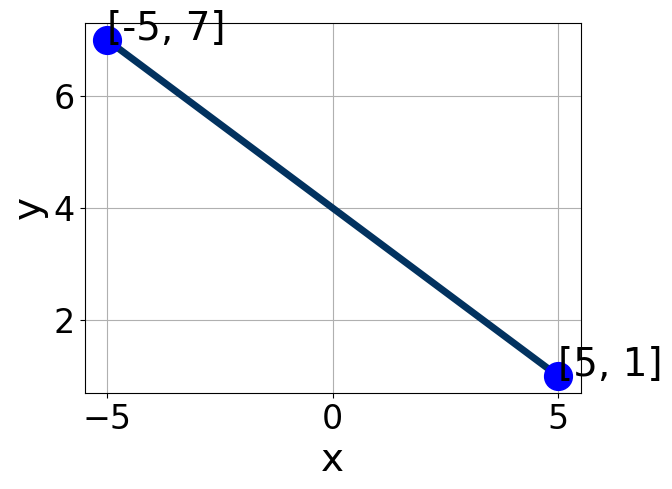
\includegraphics[width=0.5\textwidth]{../Figures/linearGraphToStandardA.png}
\end{center}
\begin{enumerate}[label=\Alph*.]
\item \( A \in [-6, -2], \hspace{3mm} B \in [-6.5, -4.1], \text{ and } \hspace{3mm} C \in [-21, -19] \)
\item \( A \in [1, 4], \hspace{3mm} B \in [-6.5, -4.1], \text{ and } \hspace{3mm} C \in [-21, -19] \)
\item \( A \in [-2.4, 2.6], \hspace{3mm} B \in [-4.5, -0.6], \text{ and } \hspace{3mm} C \in [-6, -2] \)
\item \( A \in [-2.4, 2.6], \hspace{3mm} B \in [0.5, 2.9], \text{ and } \hspace{3mm} C \in [1, 9] \)
\item \( A \in [1, 4], \hspace{3mm} B \in [3.5, 5.3], \text{ and } \hspace{3mm} C \in [19, 21] \)

\end{enumerate} }
\litem{
Solve the linear equation below. Then, choose the interval that contains the solution.\[ \frac{3x -4}{4} - \frac{5x + 6}{2} = \frac{-7x -8}{3} \]\begin{enumerate}[label=\Alph*.]
\item \( x \in [-0.2, 1.5] \)
\item \( x \in [-8.5, -6.8] \)
\item \( x \in [0.3, 3] \)
\item \( x \in [2.9, 5.1] \)
\item \( \text{There are no real solutions.} \)

\end{enumerate} }
\litem{
First, find the equation of the line containing the two points below. Then, write the equation in the form $ y=mx+b $ and choose the intervals that contain $m$ and $b$.\[ (-4, -8) \text{ and } (7, -5) \]\begin{enumerate}[label=\Alph*.]
\item \( m \in [-1.69, -0.19] \hspace*{3mm} b \in [-3.48, -3.05] \)
\item \( m \in [0.25, 0.35] \hspace*{3mm} b \in [-4.26, -3.91] \)
\item \( m \in [0.25, 0.35] \hspace*{3mm} b \in [-13.01, -11.52] \)
\item \( m \in [0.25, 0.35] \hspace*{3mm} b \in [5.35, 7.65] \)
\item \( m \in [0.25, 0.35] \hspace*{3mm} b \in [-8.14, -6.21] \)

\end{enumerate} }
\litem{
Solve the linear equation below. Then, choose the interval that contains the solution.\[ \frac{4x -5}{8} - \frac{7x -8}{5} = \frac{-4x + 7}{3} \]\begin{enumerate}[label=\Alph*.]
\item \( x \in [3.1, 3.26] \)
\item \( x \in [8.68, 9.71] \)
\item \( x \in [0.88, 1.5] \)
\item \( x \in [10.29, 11.53] \)
\item \( \text{There are no real solutions.} \)

\end{enumerate} }
\litem{
Solve the equation below. Then, choose the interval that contains the solution.\[ -16(6x -13) = -10(-4x -3) \]\begin{enumerate}[label=\Alph*.]
\item \( x \in [1.32, 2.57] \)
\item \( x \in [-1.84, -1.38] \)
\item \( x \in [3.37, 4.88] \)
\item \( x \in [1.2, 1.37] \)
\item \( \text{There are no real solutions.} \)

\end{enumerate} }
\litem{
First, find the equation of the line containing the two points below. Then, write the equation in the form $ y=mx+b $ and choose the intervals that contain $m$ and $b$.\[ (9, 2) \text{ and } (4, -4) \]\begin{enumerate}[label=\Alph*.]
\item \( m \in [0.2, 4.2] \hspace*{3mm} b \in [-9.72, -8.07] \)
\item \( m \in [0.2, 4.2] \hspace*{3mm} b \in [-7.07, -6.82] \)
\item \( m \in [-6.2, 0.8] \hspace*{3mm} b \in [0.18, 1.12] \)
\item \( m \in [0.2, 4.2] \hspace*{3mm} b \in [8.48, 10.02] \)
\item \( m \in [0.2, 4.2] \hspace*{3mm} b \in [-8.74, -7.05] \)

\end{enumerate} }
\litem{
Find the equation of the line described below. Write the linear equation in the form $ y=mx+b $ and choose the intervals that contain $m$ and $b$.\[ \text{Parallel to } 4 x + 7 y = 6 \text{ and passing through the point } (-10, 7). \]\begin{enumerate}[label=\Alph*.]
\item \( m \in [0.13, 0.63] \hspace*{3mm} b \in [10.9, 13.8] \)
\item \( m \in [-1.26, -0.23] \hspace*{3mm} b \in [15.6, 17.4] \)
\item \( m \in [-1.26, -0.23] \hspace*{3mm} b \in [-1.4, -0.3] \)
\item \( m \in [-1.26, -0.23] \hspace*{3mm} b \in [1, 2.5] \)
\item \( m \in [-1.86, -1.45] \hspace*{3mm} b \in [1, 2.5] \)

\end{enumerate} }
\litem{
Solve the equation below. Then, choose the interval that contains the solution.\[ -2(18x + 15) = -17(5x + 4) \]\begin{enumerate}[label=\Alph*.]
\item \( x \in [-0.8, -0.75] \)
\item \( x \in [-2.07, -1.94] \)
\item \( x \in [-0.85, -0.8] \)
\item \( x \in [1.97, 2.04] \)
\item \( \text{There are no real solutions.} \)

\end{enumerate} }
\litem{
Write the equation of the line in the graph below in Standard Form $Ax+By=C$. Then, choose the intervals that contain $A, B, \text{ and } C$.
\begin{center}
    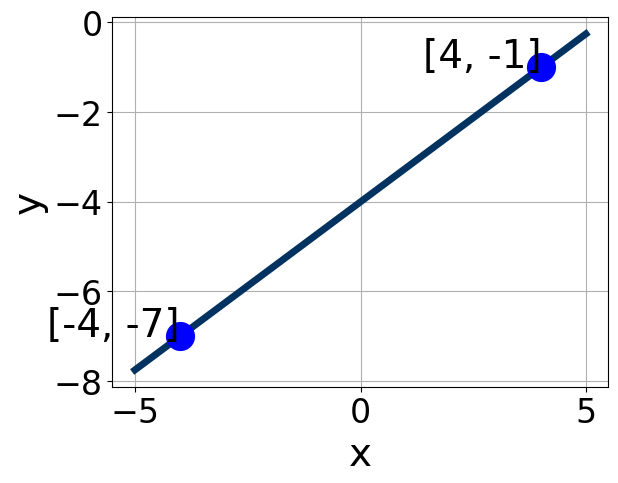
\includegraphics[width=0.5\textwidth]{../Figures/linearGraphToStandardCopyB.png}
\end{center}
\begin{enumerate}[label=\Alph*.]
\item \( A \in [0, 11], \hspace{3mm} B \in [-4.9, -2.1], \text{ and } \hspace{3mm} C \in [11, 17] \)
\item \( A \in [-5, -2], \hspace{3mm} B \in [3, 5.3], \text{ and } \hspace{3mm} C \in [-17, -13] \)
\item \( A \in [0, 11], \hspace{3mm} B \in [3, 5.3], \text{ and } \hspace{3mm} C \in [-17, -13] \)
\item \( A \in [-1.75, 1.25], \hspace{3mm} B \in [-1.9, -0.3], \text{ and } \hspace{3mm} C \in [4, 9] \)
\item \( A \in [-1.75, 1.25], \hspace{3mm} B \in [-0.9, 3.9], \text{ and } \hspace{3mm} C \in [-6, -3] \)

\end{enumerate} }
\litem{
Find the equation of the line described below. Write the linear equation in the form $ y=mx+b $ and choose the intervals that contain $m$ and $b$.\[ \text{Perpendicular to } 8 x - 7 y = 15 \text{ and passing through the point } (-8, 2). \]\begin{enumerate}[label=\Alph*.]
\item \( m \in [-0.95, -0.63] \hspace*{3mm} b \in [9.4, 12.2] \)
\item \( m \in [-0.95, -0.63] \hspace*{3mm} b \in [4.8, 7.4] \)
\item \( m \in [-0.95, -0.63] \hspace*{3mm} b \in [-5.7, -4.2] \)
\item \( m \in [-1.29, -0.91] \hspace*{3mm} b \in [-5.7, -4.2] \)
\item \( m \in [0.67, 0.93] \hspace*{3mm} b \in [8.9, 9.9] \)

\end{enumerate} }
\litem{
Write the equation of the line in the graph below in Standard Form $Ax+By=C$. Then, choose the intervals that contain $A, B, \text{ and } C$.
\begin{center}
    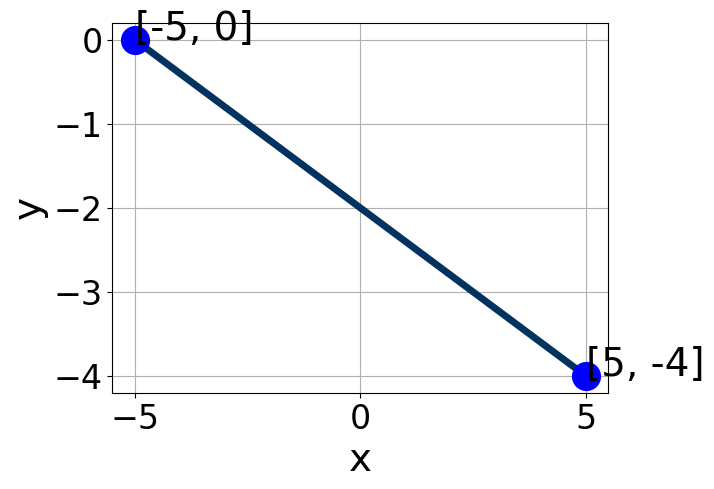
\includegraphics[width=0.5\textwidth]{../Figures/linearGraphToStandardB.png}
\end{center}
\begin{enumerate}[label=\Alph*.]
\item \( A \in [-0.74, 0.63], \hspace{3mm} B \in [-0.1, 3.7], \text{ and } \hspace{3mm} C \in [-3, 0] \)
\item \( A \in [-3.35, -0.07], \hspace{3mm} B \in [-8, -2.4], \text{ and } \hspace{3mm} C \in [10, 15] \)
\item \( A \in [0.71, 2.16], \hspace{3mm} B \in [3.6, 6.3], \text{ and } \hspace{3mm} C \in [-16, -9] \)
\item \( A \in [0.71, 2.16], \hspace{3mm} B \in [-8, -2.4], \text{ and } \hspace{3mm} C \in [10, 15] \)
\item \( A \in [-0.74, 0.63], \hspace{3mm} B \in [-2.5, 0.2], \text{ and } \hspace{3mm} C \in [1, 9] \)

\end{enumerate} }
\litem{
Solve the linear equation below. Then, choose the interval that contains the solution.\[ \frac{4x + 7}{8} - \frac{-5x -7}{4} = \frac{8x -5}{2} \]\begin{enumerate}[label=\Alph*.]
\item \( x \in [-8.12, -2.12] \)
\item \( x \in [7.44, 11.44] \)
\item \( x \in [-1.28, 1.72] \)
\item \( x \in [1.28, 4.28] \)
\item \( \text{There are no real solutions.} \)

\end{enumerate} }
\litem{
First, find the equation of the line containing the two points below. Then, write the equation in the form $ y=mx+b $ and choose the intervals that contain $m$ and $b$.\[ (5, -11) \text{ and } (-5, 4) \]\begin{enumerate}[label=\Alph*.]
\item \( m \in [0.8, 4.6] \hspace*{3mm} b \in [10.5, 16.5] \)
\item \( m \in [-2.8, -1.2] \hspace*{3mm} b \in [-22, -14] \)
\item \( m \in [-2.8, -1.2] \hspace*{3mm} b \in [5, 11] \)
\item \( m \in [-2.8, -1.2] \hspace*{3mm} b \in [-3.5, -0.5] \)
\item \( m \in [-2.8, -1.2] \hspace*{3mm} b \in [1.5, 8.5] \)

\end{enumerate} }
\litem{
Solve the linear equation below. Then, choose the interval that contains the solution.\[ \frac{5x + 4}{2} - \frac{3x -7}{8} = \frac{3x -6}{4} \]\begin{enumerate}[label=\Alph*.]
\item \( x \in [-3.7, -2.4] \)
\item \( x \in [3.3, 4.5] \)
\item \( x \in [-14.5, -11.3] \)
\item \( x \in [-2.2, -1.2] \)
\item \( \text{There are no real solutions.} \)

\end{enumerate} }
\litem{
Solve the equation below. Then, choose the interval that contains the solution.\[ -8(6x + 5) = -13(-4x + 7) \]\begin{enumerate}[label=\Alph*.]
\item \( x \in [32.18, 33.29] \)
\item \( x \in [-0.06, 0.79] \)
\item \( x \in [0.69, 2.49] \)
\item \( x \in [-1.35, -0.65] \)
\item \( \text{There are no real solutions.} \)

\end{enumerate} }
\litem{
First, find the equation of the line containing the two points below. Then, write the equation in the form $ y=mx+b $ and choose the intervals that contain $m$ and $b$.\[ (7, -11) \text{ and } (-7, -10) \]\begin{enumerate}[label=\Alph*.]
\item \( m \in [-0.11, -0.06] \hspace*{3mm} b \in [9.03, 10.59] \)
\item \( m \in [-0.11, -0.06] \hspace*{3mm} b \in [-11.27, -10.49] \)
\item \( m \in [-0.11, -0.06] \hspace*{3mm} b \in [-4.6, -1.23] \)
\item \( m \in [-0.11, -0.06] \hspace*{3mm} b \in [-18.5, -16.95] \)
\item \( m \in [0.04, 0.16] \hspace*{3mm} b \in [-9.63, -9.42] \)

\end{enumerate} }
\litem{
Find the equation of the line described below. Write the linear equation in the form $ y=mx+b $ and choose the intervals that contain $m$ and $b$.\[ \text{Perpendicular to } 8 x + 7 y = 15 \text{ and passing through the point } (3, -8). \]\begin{enumerate}[label=\Alph*.]
\item \( m \in [-0.92, -0.76] \hspace*{3mm} b \in [-6.66, -5.11] \)
\item \( m \in [0.74, 1.04] \hspace*{3mm} b \in [9.9, 11.01] \)
\item \( m \in [0.74, 1.04] \hspace*{3mm} b \in [-10.91, -9.65] \)
\item \( m \in [1.02, 1.16] \hspace*{3mm} b \in [-10.91, -9.65] \)
\item \( m \in [0.74, 1.04] \hspace*{3mm} b \in [-11.81, -10.68] \)

\end{enumerate} }
\litem{
Solve the equation below. Then, choose the interval that contains the solution.\[ -13(-8x -16) = -10(2x + 19) \]\begin{enumerate}[label=\Alph*.]
\item \( x \in [-3.24, -3.16] \)
\item \( x \in [0.01, 0.16] \)
\item \( x \in [-0.21, -0.14] \)
\item \( x \in [-0.26, -0.2] \)
\item \( \text{There are no real solutions.} \)

\end{enumerate} }
\litem{
Write the equation of the line in the graph below in Standard Form $Ax+By=C$. Then, choose the intervals that contain $A, B, \text{ and } C$.
\begin{center}
    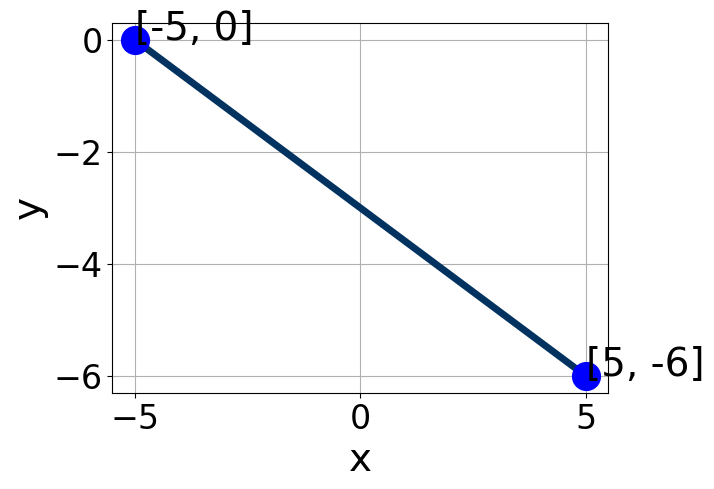
\includegraphics[width=0.5\textwidth]{../Figures/linearGraphToStandardCopyC.png}
\end{center}
\begin{enumerate}[label=\Alph*.]
\item \( A \in [0, 2.7], \hspace{3mm} B \in [-4, 0.2], \text{ and } \hspace{3mm} C \in [1, 8] \)
\item \( A \in [-3.6, -2.9], \hspace{3mm} B \in [-5.5, -3.2], \text{ and } \hspace{3mm} C \in [13, 18] \)
\item \( A \in [0.8, 3.7], \hspace{3mm} B \in [-5.5, -3.2], \text{ and } \hspace{3mm} C \in [13, 18] \)
\item \( A \in [0, 2.7], \hspace{3mm} B \in [-0.2, 2], \text{ and } \hspace{3mm} C \in [-12, 1] \)
\item \( A \in [0.8, 3.7], \hspace{3mm} B \in [3.3, 6], \text{ and } \hspace{3mm} C \in [-15, -13] \)

\end{enumerate} }
\litem{
Find the equation of the line described below. Write the linear equation in the form $ y=mx+b $ and choose the intervals that contain $m$ and $b$.\[ \text{Parallel to } 5 x - 9 y = 12 \text{ and passing through the point } (-7, -8). \]\begin{enumerate}[label=\Alph*.]
\item \( m \in [-0.28, 0.66] \hspace*{3mm} b \in [-6.11, -3.11] \)
\item \( m \in [-0.99, 0.16] \hspace*{3mm} b \in [-18.89, -10.89] \)
\item \( m \in [-0.28, 0.66] \hspace*{3mm} b \in [-3, 2] \)
\item \( m \in [1.69, 2.14] \hspace*{3mm} b \in [-6.11, -3.11] \)
\item \( m \in [-0.28, 0.66] \hspace*{3mm} b \in [2.11, 7.11] \)

\end{enumerate} }
\litem{
Write the equation of the line in the graph below in Standard Form $Ax+By=C$. Then, choose the intervals that contain $A, B, \text{ and } C$.
\begin{center}
    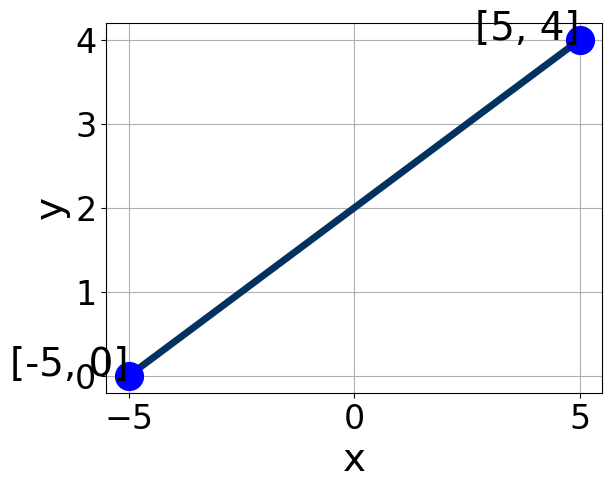
\includegraphics[width=0.5\textwidth]{../Figures/linearGraphToStandardC.png}
\end{center}
\begin{enumerate}[label=\Alph*.]
\item \( A \in [-0.63, 1.12], \hspace{3mm} B \in [-0.2, 2.36], \text{ and } \hspace{3mm} C \in [1, 6] \)
\item \( A \in [1.99, 4.03], \hspace{3mm} B \in [-5.17, -4.42], \text{ and } \hspace{3mm} C \in [-12, -6] \)
\item \( A \in [1.99, 4.03], \hspace{3mm} B \in [3.95, 6], \text{ and } \hspace{3mm} C \in [5, 17] \)
\item \( A \in [-2.3, -1.15], \hspace{3mm} B \in [3.95, 6], \text{ and } \hspace{3mm} C \in [5, 17] \)
\item \( A \in [-0.63, 1.12], \hspace{3mm} B \in [-1.75, 0.36], \text{ and } \hspace{3mm} C \in [-4, 1] \)

\end{enumerate} }
\litem{
Solve the linear equation below. Then, choose the interval that contains the solution.\[ \frac{4x -3}{3} - \frac{6x + 7}{5} = \frac{3x -9}{2} \]\begin{enumerate}[label=\Alph*.]
\item \( x \in [-0.13, 0.75] \)
\item \( x \in [-1.8, -0.58] \)
\item \( x \in [2.51, 3.64] \)
\item \( x \in [0.71, 1.83] \)
\item \( \text{There are no real solutions.} \)

\end{enumerate} }
\litem{
First, find the equation of the line containing the two points below. Then, write the equation in the form $ y=mx+b $ and choose the intervals that contain $m$ and $b$.\[ (-4, 9) \text{ and } (4, 3) \]\begin{enumerate}[label=\Alph*.]
\item \( m \in [-2.1, -0.3] \hspace*{3mm} b \in [4.1, 7.43] \)
\item \( m \in [-2.1, -0.3] \hspace*{3mm} b \in [-1.77, -0.34] \)
\item \( m \in [0.2, 2.7] \hspace*{3mm} b \in [-0.68, 0.44] \)
\item \( m \in [-2.1, -0.3] \hspace*{3mm} b \in [-7.52, -3.78] \)
\item \( m \in [-2.1, -0.3] \hspace*{3mm} b \in [12.59, 13.66] \)

\end{enumerate} }
\litem{
Solve the linear equation below. Then, choose the interval that contains the solution.\[ \frac{-7x + 7}{2} - \frac{-4x + 9}{3} = \frac{-5x -7}{7} \]\begin{enumerate}[label=\Alph*.]
\item \( x \in [-2.2, 0.9] \)
\item \( x \in [1.4, 3.9] \)
\item \( x \in [0.7, 2.3] \)
\item \( x \in [5.1, 6] \)
\item \( \text{There are no real solutions.} \)

\end{enumerate} }
\litem{
Solve the equation below. Then, choose the interval that contains the solution.\[ -6(-18x + 3) = -10(-15x + 19) \]\begin{enumerate}[label=\Alph*.]
\item \( x \in [4.67, 5.4] \)
\item \( x \in [0.28, 1.26] \)
\item \( x \in [2.94, 4.46] \)
\item \( x \in [-6.68, -4.65] \)
\item \( \text{There are no real solutions.} \)

\end{enumerate} }
\litem{
First, find the equation of the line containing the two points below. Then, write the equation in the form $ y=mx+b $ and choose the intervals that contain $m$ and $b$.\[ (9, -10) \text{ and } (3, 11) \]\begin{enumerate}[label=\Alph*.]
\item \( m \in [-4.5, -1.5] \hspace*{3mm} b \in [-21.5, -20.5] \)
\item \( m \in [-4.5, -1.5] \hspace*{3mm} b \in [-20, -18] \)
\item \( m \in [-4.5, -1.5] \hspace*{3mm} b \in [16.5, 24.5] \)
\item \( m \in [-4.5, -1.5] \hspace*{3mm} b \in [5, 16] \)
\item \( m \in [-2.5, 12.5] \hspace*{3mm} b \in [0.5, 2.5] \)

\end{enumerate} }
\end{enumerate}

\end{document}